\section{Thursday, October 30th 2025}

\subsection{Introduction to Hypothesis Testing}

\begin{itemize}
    \item Recall the Neyman-Pearson test that we ended last class talking about.
    \item Hypothesis testing: the test statistic is a function of data.
    \item Null hypothesis $H_0$, alternative hypothesis $H_A$.
    \item The main idea from Neyman and Pearson was to include a second hypothesis $H_A$.
\end{itemize}

\begin{table}[h]
    \centering
    \begin{tabular}{c|c|c}
                     & $H_0$ true       & $H_A$ true       \\
        \hline
        Accept $H_0$ & Correct decision & Type II error    \\
        \hline
        Reject $H_0$ & Type I error     & Correct decision \\
    \end{tabular}
    \caption{Outcomes of hypothesis testing.}
\end{table}

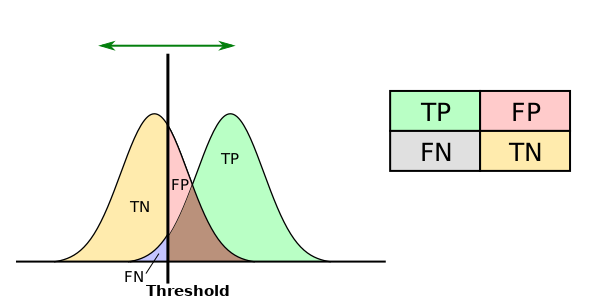
\includegraphics[width = 0.6\linewidth]{Images/lec15-neym-pear.png}

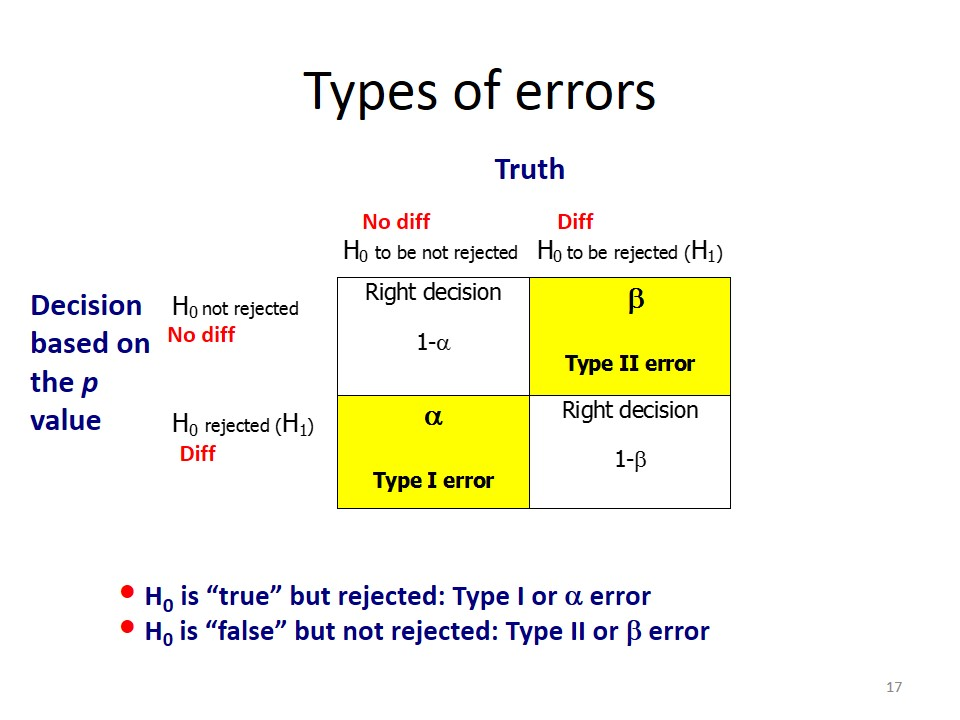
\includegraphics[width = \linewidth]{Images/lec15-type-errors.jpg}

\begin{itemize}
    \item Null Hypothesis Significance Testing (NHST).
\end{itemize}

\subsection{The Neyman-Pearson Lemma and Optimal Test Regions}

\begin{itemize}
    \item NP test: How to optimize the region $R$ to minimize Type II error for a fixed Type I error rate $\alpha$.
          \[ 1- \beta = \int_{R} P_{A}(x) \, dx \]
    \item If we move a point $x_1$ by $\delta x_1$ from $R$ to $\bar{R}$, it must be replaced by another point $x_2$ such that $\delta_{2}P_{H}(x_2) = \delta_{1} P_{H}(x_1)$. (Gain to loss condition.)
          \[ \int_{R} P_{H} = \alpha \]
    \item Then change in $1-\beta$ is $\delta_{2} P_{A} (x_2) - \delta_{1} P_{A} (x_1)$ (gain to loss).
    \item Select $R$ by picking $x$ values that maximize $P_{A}(x)/P_{H_{0}}(x)$ until $\alpha$ is reached:
          \[ \frac{\delta_{2} P_{A}(x_2)}{ \delta_{2} P_{H_{0}}(x_2)} \geq \frac{\delta_{1} P_A(x_1)}{\delta_{1} P_{H_{0}}(x_1)} \]
    \item Decision rule:
          \[ \frac{P_{A}(x)}{P_{H_{0}}(x)} \geq c_{\alpha} \]
    \item For some fixed $\alpha$, set the region by
          \[ \frac{P_{A}(x)}{P_{H_{0}}(x)} = c_{\alpha} \]
    \item i.e.
          \[ \frac{L(\vec{x}|H_{A})}{L(\vec{x}|H_{0})} \geq c_{\alpha} \]
\end{itemize}

\subsection{Gaussian Example: Testing Mean Values}

\begin{itemize}
    \item Example: data Gaussian with $\sigma = 1$.
          \[ f(x) = \frac{1}{\sqrt{2 \pi}} e^{-\frac{(x-\mu)^2}{2}} \]
    \item Our hypotheses:
          \[ H_{0}: \mu = \mu_0 \]
          \[ H_{A}: \mu = \mu_1 \]
    \item $n$ measurements:
          \[ \mathcal{L}(\vec{x} | H_{0}) = \prod_{i=1}^{n} f(x_i) = \left( \frac{1}{\sqrt{2 \pi}} \right)^n e^{-\sum_{i=1}^{n} \frac{(x_i - \mu)^2}{2}} \]
    \item Sample mean:
          \[ \bar{x} = \frac{1}{n} \sum_{i=1}^{n} x_i \]
    \item Variance of sample mean:
          \[ V(\bar{x}) = \frac{\sigma^2}{n} = \frac{1}{n} \]
    \item Sample variance:
          \[ S^2 = \frac{1}{n} \sum_{i=1}^{n} (x_i - \bar{x})^2 \]
    \item Expansion:
          \[ \sum (x_i - \mu_0)^2 = n \left((\bar{x} - \mu_0)^2 + S^2 \right) \]
    \item Likelihood ratio:
          \[ \frac{\mathcal{L}(\vec{x}|H_{1})}{\mathcal{L}(\vec{x}|H_{0})} = e^{-\frac{n}{2} \left( (\bar{x} - \mu_1)^2 - (\bar{x} - \mu_0)^2 \right)} \geq c_{\alpha} \]
          \[ \frac{n}{2} \left( 2 \bar{x} (\mu_1 - \mu_0) + \mu_1^2 - \mu_0^2 \right) \geq \ln(c_{\alpha}) \]
          \[ (\mu_1 - \mu_0) \bar{x} \geq \frac{2}{n} \ln(c_{\alpha}) + \frac{1}{2} (\mu_1^2 - \mu_0^2) \]
    \item Take the case $\mu_1 > \mu_0$:
          \[ \bar{x} \geq \frac{1}{\mu_1 - \mu_0} \left( \frac{2}{n} \ln(c_{\alpha}) + \frac{1}{2} (\mu_1^2 - \mu_0^2) \right) \]
    \item This is a Simple Statistic (and in our case it is a Sufficient Statistic as well).
    \item The distribution of $\bar{x}$ is Gaussian about the true mean with width $\sigma / \sqrt{n} = \frac{1}{\sqrt{n}}$.
    \item So:
          \[ \int_{R} \mathcal{L}(\vec{x}|H_{0}) d\vec{x} = \int_{\bar{x}_{\alpha}}^{\infty} \frac{1}{\sqrt{2 \pi}} e^{-\frac{n}{2} (\bar{x} - \mu_0)^2} d\bar{x} = \alpha \]
\end{itemize}

\subsection{Applied Example: Mineral Density Classification}

\begin{itemize}
    \item Example: Mining.
    \item Opal density = $2.2$ g/cm$^3$.
    \item Quartz density = $2.6$ g/cm$^3$.
    \item Sample standard deviation $\sigma = 0.2$ g/cm$^3$.
    \item Gaussian hypotheses:
          \begin{itemize}
              \item $H_{0} \sim N(2.2, \sigma^2)$
              \item $H_{A} \sim N(2.6, \sigma^2)$
          \end{itemize}
    \item Likelihood ratio:
          \[
              \frac{L(p|H_{A})}{L(p|H_{0})}
              = \frac{ \frac{1}{\sqrt{2 \pi \sigma^2}} e^{-\frac{(p - 2.6)^2}{2 \sigma^2}} }
              { \frac{1}{\sqrt{2 \pi \sigma^2}} e^{-\frac{(p - 2.2)^2}{2 \sigma^2}}}
              = e^{-\frac{1}{2 \sigma^2} \left( (p - 2.6)^2 - (p - 2.2)^2 \right)} \geq c_{\alpha}
          \]
    \item Cut off at $p \leq 2.56$ (which corresponds to $1.64\sigma$) so we keep $95\%$ of opals.
    \item But needlessly investigate $36\%$ of useless mines.
\end{itemize}

\subsection{Common Misconceptions in Hypothesis Testing}

\begin{itemize}
    \item A common misconception: if $P(H_{0}|x)$ is small, then $P(x|H_{0})$ must be small. This is \textbf{not true}.
    \item Example: $P(\text{American} | \text{walked on moon}) = 1$, but $P(\text{walked on moon} | \text{American})$ is very small.
\end{itemize}
